% Copyright (C)  2015  Alexander Jankowski, Philipp Hacker.
% Permission is granted to copy, distribute and/or modify this document
% under the terms of the GNU Free Documentation License, Version 1.3
% or any later version published by the Free Software Foundation;
% with no Invariant Sections, no Front-Cover Texts, and no Back-Cover Texts.
% The lincense itself can be found at <https://www.gnu.org/licenses/fdl-1.3>.

\documentclass[numbers=noenddot,a4paper,notitlepage,twoside,BCOR15mm]{scrartcl}
%\documentclass[numbers=noenddot,12pt,a4paper]{scrartcl}

\usepackage{ifoddpage}
\usepackage[infoshow]{tabularx}
\usepackage{fancyhdr}
\usepackage[greek,ngerman]{babel}
\usepackage[T1]{fontenc}
\usepackage[utf8]{inputenc}
\usepackage{libertine}
\usepackage{ziffer}
\usepackage{graphicx}
\usepackage{units}
\usepackage[infoshow]{tabularx}
\usepackage[all]{xy}
\usepackage{amsmath}
\usepackage{amssymb}
\usepackage{wrapfig}
\usepackage{upgreek}
\usepackage{esint}
\usepackage{float}
\usepackage[font=small,labelfont=bf]{caption}
\usepackage{subcaption}
\usepackage{lscape}
\usepackage[backref=page]{hyperref}
\usepackage{cleveref}
\usepackage{csquotes}

\renewcommand{\headrulewidth}{0.1pt}
\renewcommand{\footrulewidth}{0.1pt}
\newcommand{\name}{\text{Philipp Hacker}} %TODO Name des Protokollanten eintragen

\renewcaptionname{ngerman}{\figurename}{Abb. }
\renewcaptionname{ngerman}{\tablename}{Tab.}

\setlength{\parindent}{0pt}

\newcommand{\nummat}[1]{\left[\text{#1}\right]}
\newcommand{\num}[1]{$\left[\text{#1}\right]$}
\newcommand{\degree}{^\circ}
\newcommand{\diff}{\textnormal{d}}
\newcommand{\tenpo}[1]{ 10^{#1}}
\newcommand{\greek}[1]{\greektext#1\latintext}
\newcommand{\ix}[1]{_\text{#1}}
\newcommand{\imag}{\mathbf{i}}
\newcommand{\tilt}[1]{\textit{#1}}
\newcommand{\grad}[1]{\textit{grad}\left(#1\right)}
\newcommand{\divergenz}[1]{\textit{div}\left(#1\right)}
\newcommand{\euler}{\mathnormal{e}}
\newcommand{\fett}[1]{\textbf{#1}}
\newcommand{\einnup}{\hspace{0.2cm}}
\newcommand{\einnum}{\hspace{-0.2cm}}
\newcommand{\zentriert}[1]{\begin{center}#1\end{center}}

\title{Protokoll: Mie-Streuung} %TODO Name des Versuchs eintragen
\author{Alexander Jankowski, Philipp Hacker}
\date{\today}
\pagestyle{fancy}
\fancyhead[C]{\thepage}
\fancyhead[R]{\name}
\fancyfoot[C]{\thepage}
\fancyhead[L]{Abschnitt \thesection}

\begin{document}
	\maketitle
	\begin{center}
		Betreuer: Malte Paßvogel\\ %TODO Name des Betreuers eintragen
		Versuchsdatum: 28./29.10.2015\\ %TODO Datum des Versuchs eintragen
		\begin{table}[h]
			\centering
			Note: %TODO Gute Note erhalten :)
			\begin{tabularx}{1.5cm}{|X|}
				\hline \\ \\
				\hline
			\end{tabularx}
		\end{table}
	\end{center}
	\vspace*{\fill}
	\tableofcontents
	\vfill
	\newpage
	\section{Motivation}

	\newpage
	\section{Physikalische Grundlagen}

		\subsection{Streutheorie elektromagnetischer Wellen nach Mie}\label{subsec:miestreu}

			Die Theorie der \tilt{Mie-Streuung} (oder auch \tilt{Lorenz-Mie-Streuung}) wurde von Gustav Mie 1908 - während seiner Professur an der Ernst-Moritz-Arndt-Universität in Greifswald - eingeführt und beschäftigt sich mit der elastischen Streuung von elektromagnetischen Wellen an sphärischen Objekten, deren Dimension i.A. etwa der Länge eines Wellenzuges entspricht. Konkreter handelt es sich dabei um die exakte Lösung der n Maxwell-Gleichungen für ebene Lichtwellen, die auf ein Teilchen treffen, welches unter der Einwirkung dieser externen Felder Mutlipolmomente der Elektronenkonfiguration ausbildet. Man versteht - grob gesagt - die einfallende elektromagnetische Welle als Störung der ruhenden Elektronenwolke des \tilt{targets}, welche dann, unter Reflexion, Absorption und Brechung wieder eine Welle emittiert, die mit den Multipolmomenten moduliert ist. Schließlich erhält man als ausfallende Welle abstrahlende, sphärische Wellenfunktionen (e.g. Kugelflächenfunktionen) und als Feld des Partikels einfache sphärische Flächenfunktionen. Die damit an jedem Raumpunkt berechenbare Welle ergibt sich als Interferenzerscheinung der vom Objekt gebeugten Teilwellen, wie sie die Ladungsträgerschwankungen moduliert hatten.\\
			Die Mie-Streuung ist, in Relationen zur Wellenlänge $\lambda$ des eingestrahlten Lichtes, im Bereich von $\unit[0,2]{\lambda}<R<\unit[2]{\lambda}$ des Radius $R$ des Partikels eine gute Möglichkeit, das Lichtfeld um z.B. ein Kolloid zu beschreiben. Dementsprechend kann man aus der Untersuchung dessen auf verschiedenste Eigenschaften des Objektes schließen: Elektronendichten bzw. -verteilungen, Größe, Beschaffenheit und daraus folgend Brechungsindex, Absorption usw.\\
			Um der Theorie eine mathematische Struktur zu geben, seien einige Ausdrücke für spektroskopische Größen angeführt.\\
			Die Absorption $\varepsilon\ix{Im}=\text{Im}\left(\varepsilon\left(\omega\right)\right)$ und die Polarisation einer Welle $\varepsilon\ix{Re}=\text{Re}\left(\varepsilon\left(\omega\right)\right)$ sind die Anteile der dielektrischen Funktion $\varepsilon\left(\omega\right)$ des Partikels, wobei $\omega$ die Frequenz des Eingestrahlten Lichtes ist, $\omega\ix{P}$ die Plasma-Frequenz und $\Gamma=v\ix{F}/\lambda\ix{mfp}$ die Dämpfung mit der Fermi-Geschwindigkeit $v\ix{F}$.

				\begin{align}
					\varepsilon\left(\omega\right)=1-\frac{\omega\ix{P}^2}{\omega^2-\imag\Gamma\omega}
				\end{align}

				Dabei versteht sich diese dielektrische Reaktion des (metallischen) Kolloids als Wechselwirkung der quasi-freien Elektronen des Clusters mit der Welle.\\
				Die Brechung durch Streuung am \tilt{target} sei $\tilde{n}\left(\omega\right)=\sqrt{\varepsilon\left(\omega\right)}=n\left(\omega\right)+\imag\kappa\left(\omega\right)$ mit

					\begin{align}
						n\left(\omega\right),\, \kappa\left(\omega\right)= \sqrt{\pm\frac{\varepsilon\ix{Re}}{2}+\frac{\sqrt{\varepsilon\ix{Re}^2+\varepsilon\ix{Im}^2}}{2}}\,\,. \label{eq:kappan}
					\end{align}

				Mit diesen Größen kann, in Zusammenhang mit dem \tilt{Lambert-Beer}'schen Extinktionsgesetz, die Absorption $\gamma\left(\lambda\right)$ der Partikel bestimmt werden. Setzt man die Auslöschung exponentiell über eine Kolloid-Dichte $\rho$, den Extinktionsquerschnitt $\sigma\ix{Ext}$ und die Strecke $D$ des Durchlaufs an, so erhält man

				\begin{align}
					I=I\ix{0}\exp\left(-\gamma\left(\lambda\right)D\right)=I\ix{0}\exp\left(-\rho\sigma\ix{Ext}D\right) \\
					\gamma\left(\lambda\right)=\frac{4\pi\kappa\left(\lambda\right)}{\lambda}=-N\sigma\ix{Ext}=\frac{1}{D}\ln\left(\frac{I\ix{0}}{I}\right) \label{eq:extinkt-intens} \,\,.
				\end{align}

			Die \autoref{eq:extinkt-intens} ist dabei wichtig für die experimentelle Bestimmung des relevanten Querschnitts und der damit zusammenhängenden Absorption, weil diese über den \tilt{logarithmus naturalis} einfach zu ermitteln sind. Das verwendete $\sigma\ix{Ext}=\sigma\ix{Abs}+\sigma\ix{Streu}$ setzt sich aus 2 getrennten Koeffizienten für die Streuung und Absorption zusammen. Stellt man nach $\sigma\ix{Abs}$ um, dh. $\sigma\ix{Abs}=\sigma\ix{Ext}-\sigma\ix{Streu}$, so gilt für diese die Entwicklung nach sphärisch-harmonischen Multipolmomenten $a\ix{L}$ und $b\ix{L}$ , welche wiederum explizit vom Imaginär- und Realteil der dielektrischen Funktion $\varepsilon\left(\omega\right)$ abhängen - hierbei ist $\varepsilon\ix{m}$ die Dielektrizität des umgebenden \tilt{bulks}.

				\begin{align}
					\sigma\ix{Ext}=&\frac{\lambda^2}{2\pi\varepsilon\ix{m}}\sum_{L}\left(-1\right)^{L}\text{Im}\left(a\ix{L}-b\ix{L}\right)\\
					\sigma\ix{Streu}=&\frac{\lambda^2}{2\pi\varepsilon\ix{m}}\sum_{L}\frac{|a\ix{L}|^2-|b\ix{L}|^2}{2L+1}
				\end{align}

			Die Extinktion der Welle mit $R\ll\lambda$ wird durch den elektrischen Streukoeffizienten $a\ix{L}$ der 1. Ordnung - die dipolare Partialwelle - dominiert. Die Streuung an den Multipolfeldern des Kolloids und insbesondere dessen magnetischen Momenten kann vernachlässigt werden, e.g. $\sigma\ix{Streu}\approx0$\,. Daraus folgt, dass der Absoprtions-Querschnitt näherungsweise durch den Dipol-Ausdruck des Extinktions-Parameters beschrieben werden kann

				\begin{align}
					\sigma\ix{Ext}^{Dip}\left(\lambda\right)=\frac{24\pi^2 R^3}{\lambda}\frac{\varepsilon\ix{m}^{\frac{3}{2}}\varepsilon\ix{Im}\left(\lambda\right)}{\left(\varepsilon\ix{Re}\left(\lambda\right)+2\varepsilon\ix{m}\right)^2+\varepsilon\ix{Im}^{2}\left(\lambda\right)}
				\end{align}

			Man erhält nach dieser Formel also eine maximale Extinktion - das Resonanzverhalten des Kolloids mit der einfallenden Welle - für ein Minimum des Nenners, e.g. $|\varepsilon\left(\lambda\right)+2\varepsilon\ix{m}|\leftarrow\text{min}$\,.\\
			Bisher wurde auf Basis der Mie-Theorie von einem quasi-statischen Modell, welches nur ein einzelnes Partikel mit freien Elektronen in einem Medium mit $\varepsilon\ix{m}$ betrachtet, ausgegangen. Um die Veränderungen des umliegenden \tilt{bulks} nicht zu vernachlässigen, fügt man den Füllfaktor $f=4/3\pi R^3\rho$ ein, welcher der endlichen Zahl von nächsten Kolloiden in einer Suspension Rechnung trägt. Diese beeinflussen offensichtlich die Randbedingungen der sog. \tilt{Plasmonenschwingungen} und dürfen für reale System demnach nicht vernachlässigt werden.\\
			Man führt des weiteren die \tilt{Lorentz-Kugel} ein, welche eine derart gewählte Dimension hat, sodass das \tilt{bulk} außerhalb als homogen angenommen werden kann. Daraus folgt, dass ebenso die Felder dort quasi-kontinuierlich sind. Der Einfluss jener Kolloide, welche hinter der Oberfläche der Kugel liegen, wird durch das effektive Feld bzw. die effektive dielektrische Funktion $\varepsilon\ix{eff}\left(\lambda\right)$ des Mischmediums beschrieben. Letztendlich ist das Ergebnis der Wechselwirkung zwischen den Partikeln gleich dem $\rho$-fachen des Einflusses eines einzelnen Teilchens (für $f<\tenpo{-3}$):

				\begin{align}
					\gamma\left(\lambda\right)=\rho\sigma\ix{Ext}^{Dip}=\frac{18\pi}{\lambda}f\frac{\varepsilon\ix{m}^{\frac{3}{2}}\varepsilon\ix{Im}\left(\lambda\right)}{\left(\varepsilon\ix{Re}\left(\lambda\right)+2\varepsilon\ix{m}\right)^2+\varepsilon\ix{Im}^{2}\left(\lambda\right)}
				\end{align}

			Für größere Füllfaktoren kann man zusammen mit \autoref{eq:effektdielektr} und \autoref{eq:maxwellgarnett} (dem \tilt{Maxwell-Garnett-Koeffizieten}) auch Probleme mit höherer Kolloid-Dichte beschreiben. Schließlich lassen sich mit \autoref{eq:extinkt-intens}, \autoref{eq:kappan} und der effektiven dielektrischen Funktion $\varepsilon\ix{eff}\left(\lambda\right)$ unter Vergleich mit experimentell gewonnenen Daten die Absorptions- und Extinktionsgrößen $\kappa$, $\gamma$ und $\sigma\ix{Ext}^{Dip}$ bestimmt werden.

				\begin{align}
					\varepsilon\ix{eff}\left(\lambda\right)=\varepsilon\ix{m}\frac{1+2f\Lambda\ix{MG}}{1-f\Lambda\ix{MG}} \label{eq:effektdielektr}\\
					\Lambda\ix{MG}\left(\lambda\right)=\frac{\varepsilon\left(\lambda\right)-\varepsilon\ix{m}}{\varepsilon\left(\lambda\right)+2\varepsilon\ix{m}} \label{eq:maxwellgarnett}
				\end{align}


		\subsection{Atomic-Force-Microscopy (Rasterkraftmikroskop)}\label{subsec:afm}

				\begin{wrapfigure}{r}{0.4\textwidth}
					\centering
					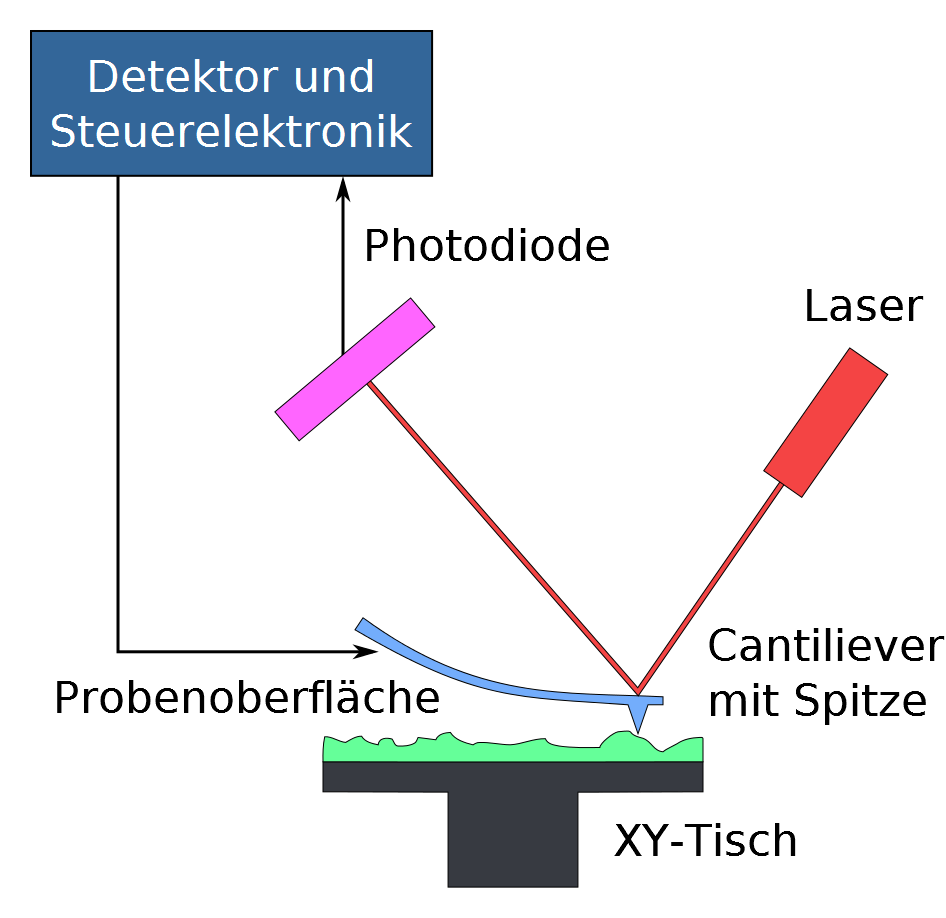
\includegraphics[width=0.4\textwidth]{Atomic_force_microscope_block_diagram_(de).png}
					\caption{Aufbau einer AFM \cite{Wiki:AFM}}
				\end{wrapfigure}

			Bei dieser Messmethode wird mit einem sog. \tilt{Cantilever} (Blattfeder) und einer daran befestigten Nanometer-großen Nadel eine diskretisierte Oberfläche abgerastert. Die Rasterung mit Hilfe von Piezo-Elementen kann hauptsächlich auf 3 Arten der Lagerung von Spitze zur Probe erfolgen: Kontakt, Nicht-Kontakt und intermittierend. Aufgrund der Wechselwirkung (atomare Kräfte, \tilt{atomic forces}) Spitze-Oberfläche biegt sich der feine Cantilever unterschiedlich stark. Diese Verbiegung kann auf verschiedene Weisen - piezo-elektronische Verfahren, optische/interferometrische Messung oder kapazitive Steuerung - gemessen werden, wodurch auf das Profil der Probe geschlossen wird. Bei den erwähnten atomaren Kräften geht es für größere Abstände (einige Mirko-Meter) um die langreichweitigen, anziehenden \tilt{Van-der-Waals-} und Kappillarkräfte. Für Entfernungen Spitze-Oberfläche von wenigen Nano-Metern üben die kurzreichweitigen, abstoßenden Austausch- (auf Grund der Überlappung von Orbitalen der Atome in der Spitze und Oberfläche) und Coulomb-Wechselwirkung einen größeren Einfluss auf die Cantilever-Biegung aus.\\
			Beim Kontakt-Modus der Messung steht die Spitze in direktem, mechanischen Kontakt zur Probe. Die voranging erfahrene Kraft am Cantilever kommt aus der Coulomb-Abstoßung. Einerseits kann man dabei für eine konstante Höhe der Nadel, oder, in Zusammenarbeit mit einem Piezo-Steuerelement, eine konstante Kraft auf diese und somit entsprechende Verbiegung des Cantilevers rastern.\\
			Im Nicht-Kontakt-Modus wird die Feder elektrisch zur Schwingung mit ihrer Resonanz-Frequenz angeregt. Die Frequenz-Antwort des Cantilevers bei der Wechselwirkung mit der Oberfläche kann als Dämpfung aufgefasst werden. Diese Frequenz-Verschiebung Damit gewinnt man Informationen über die Beschaffenheit der Probe.\\
			Während des Intermittierenden Modus oder auch \tilt{tapping mode} wird, ähnlich wie zuvor, die Anregung des Cantilevers nahe seiner Resonanz vorgenommen. Die Regelung des Schwingkreises, die Amplitude der Spitzen-Schwingung konstant zu halten, liefert eine Veränderung des Abstandes und damit Anpassung an die Kraftwechselwirkung mit der Oberfläche. Diese Betriebsart ist ideal für Proben mit empfindlichen Strukturen, die möglicherweise nicht beschädigt werden sollen. Insbesondere liefert der tapping mode die besten Ergebnisse (im Hinblick auf Verfälschung der Messung), da dieser die Kolloide in diesem Versuch nicht verschiebt oder - stellt man sich eine Kugel, welche über eine andere Kugel hinweg läuft (idealisiert) vor, so entsteht ein gewisser Fehler auf Basis ihrer Radien und geometrischen Formen - einen systematischen Fehler mit sich bringt.

				\begin{figure}[t]
					\centering
					\begin{subfigure}{0.48\textwidth}
						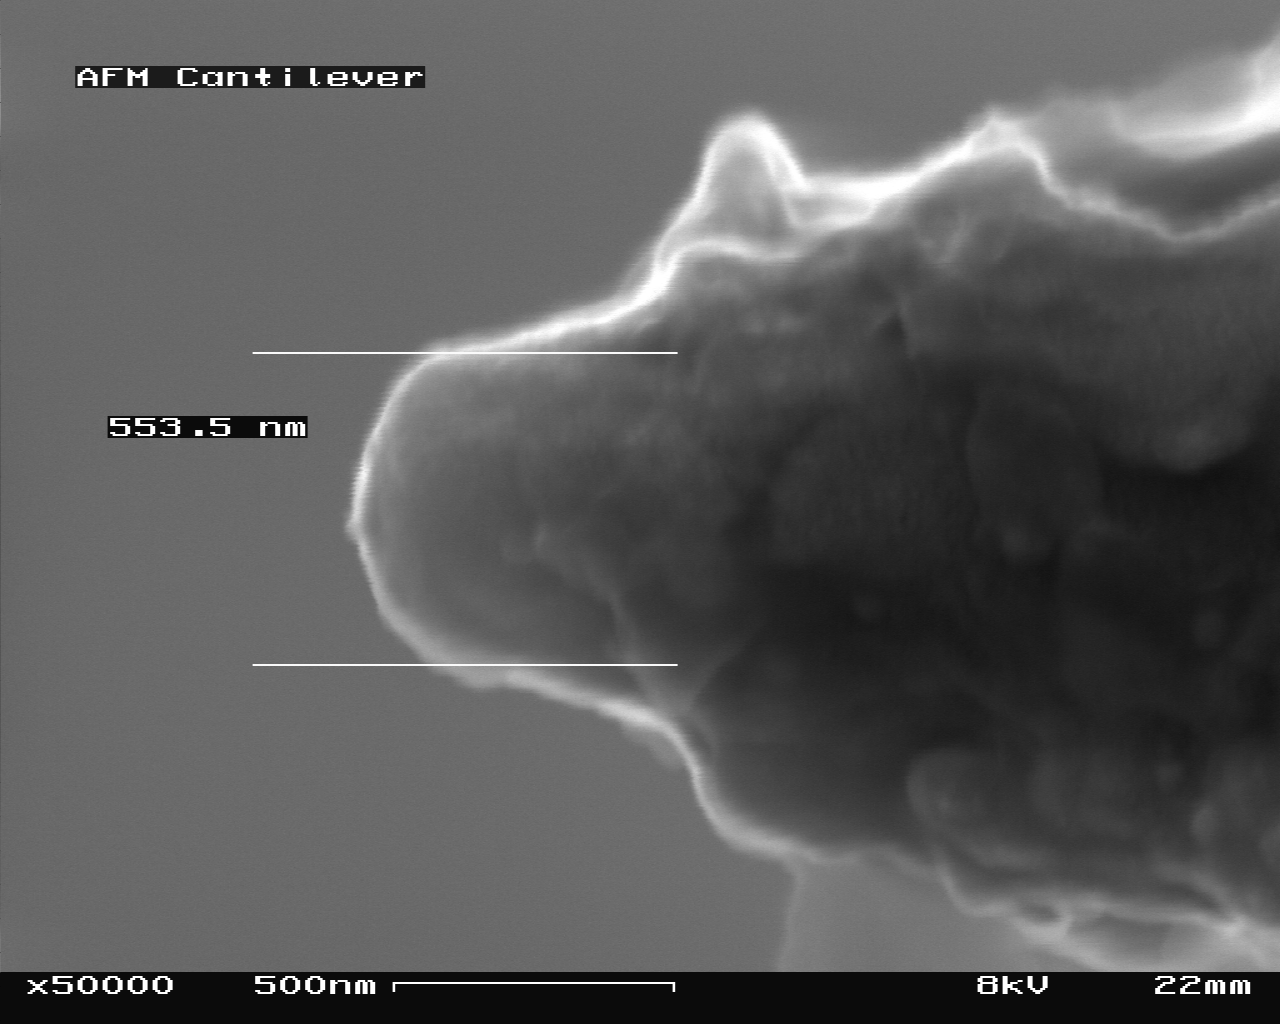
\includegraphics[width=\textwidth]{AFM_(used)_cantilever_in_Scanning_Electron_Microscope,_magnification_50000x.png}
						\caption{}
					\end{subfigure}
					\begin{subfigure}{0.48\textwidth}
						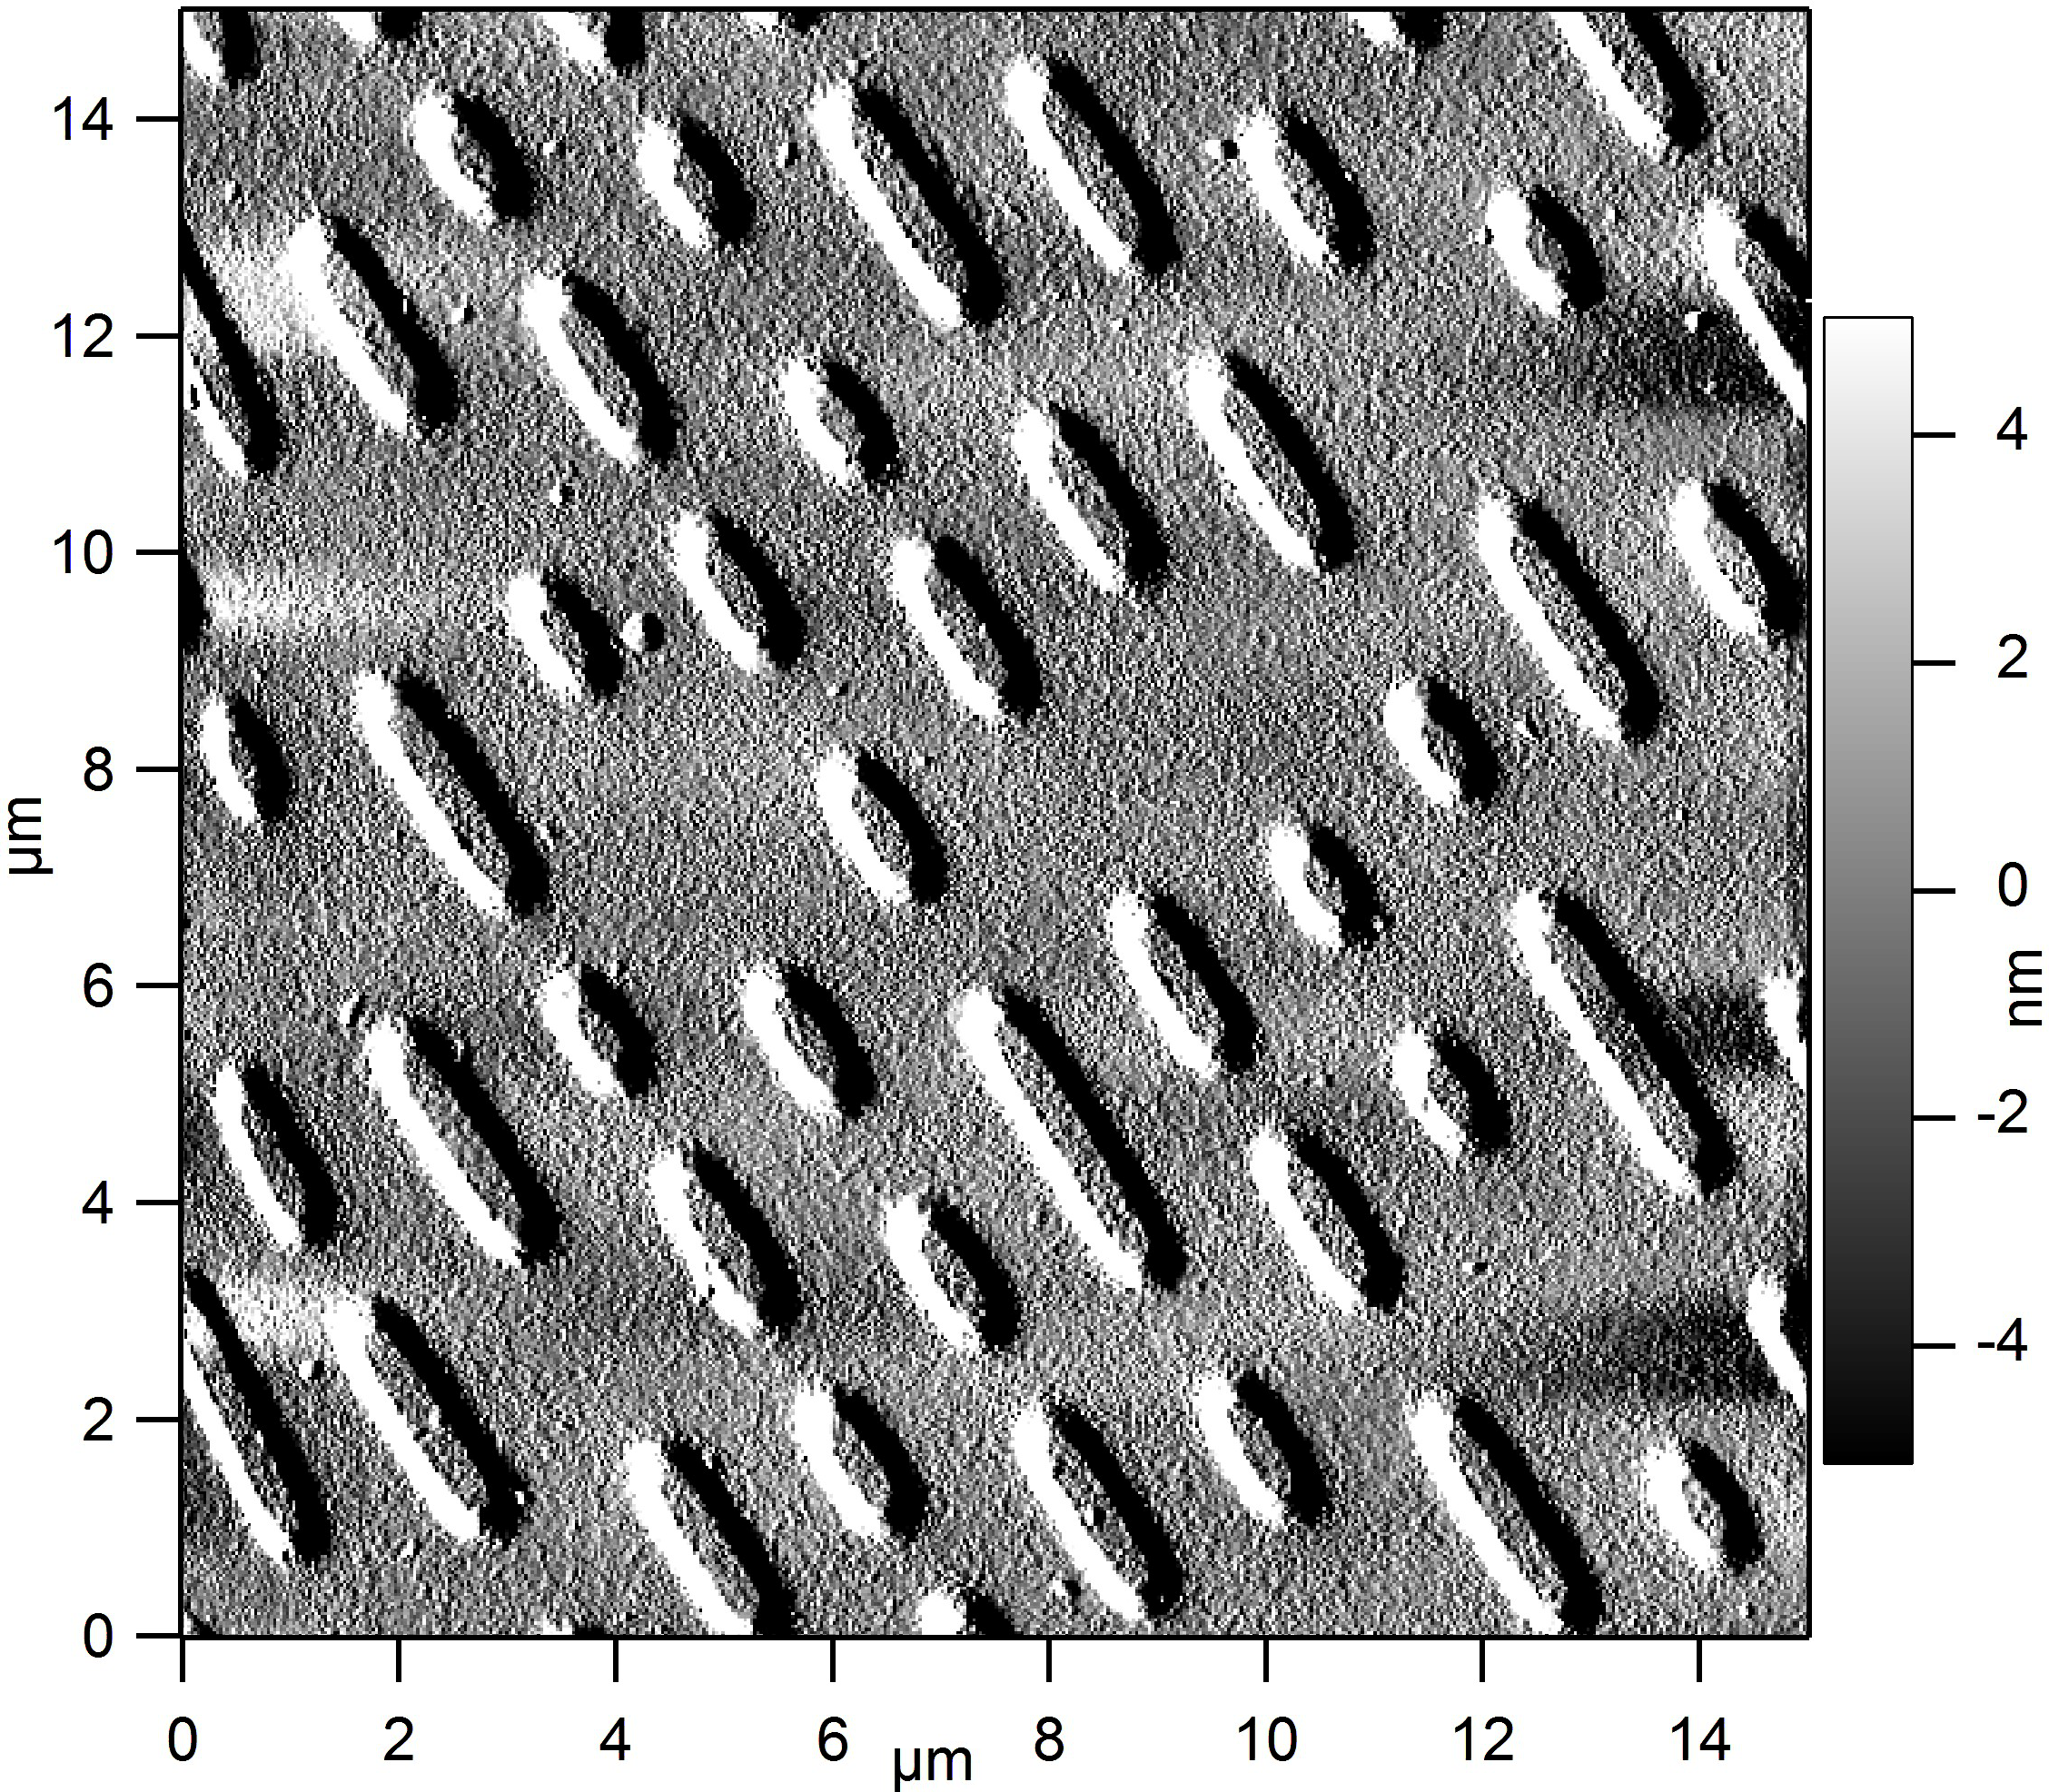
\includegraphics[width=\textwidth]{Afm_cd-rom.png}
						\caption{}
					\end{subfigure}
					\caption{\textbf{(a)}: Benutzte AFM-Spitze, Elektronenmikroskop-Aufnahme \textbf{(b)}:AFM-Aufnahme einer CD-ROM \cite{Wiki:AFM}}
				\end{figure}

		\subsection{Röntgenreflektometrie}\label{subsec:röntgen}

				\begin{figure}[t]
					\centering
					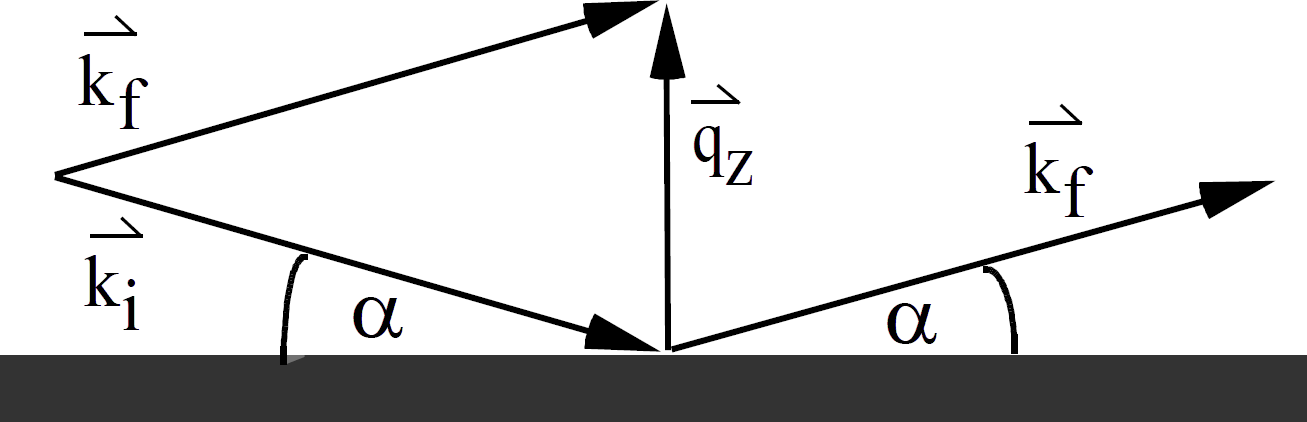
\includegraphics[width=0.55\textwidth]{rontgen2.png}
					\caption{Schema der Reflektion von Röntgenstrahlung an einer nicht-glatten Oberfläche \cite{EMAUGreifswaldMIE}}
				\end{figure}

			Die Röntgenflektometrie ist eine analytische, spektroskopische Oberflächenuntersuchung, bei der man sich den Eigenschaften von Röntgenstrahlen und dessen Streuung an dünnen Schichten mit nicht perfekt glatter Struktur zu Nutze macht.\\
			Dabei beobachtet man, die unter einem sehr flachen Einfallswinkel eintreffenden Röntgenstrahlen nach ihrer Reflexion. Dem \tilt{Senllius'schen Brechungsgesetz} zur Folge geht man davon aus, dass das Maximum dessen Intensität beim Einfallswinkel liegt - man verwendet daher ein sog. \tilt{Goniometer} ($2\vartheta$-Anordnung). Weicht die Struktur von der gemachten Forderung ab, so stimmen auch nicht mehr die von den \tilt{Fresnel-Gleichungen} vorhergesagten Intensitäten mit den gemessenen überein. Dies ist insbesondere für genügende Messgenauigkeit immer der Fall.\\
			Mit der Idee, dass in der Röntgenoptik der Brechnungsindex wie \autoref{eq:brechung} geht und das die Reflexion - im speziellen also Transmission, Emission und daraus folgend Absorption - von der elektronischen Struktur der Oberfläche abhängt, ergibt sich grundlegend für das Verhältnis aus gemessener Reflektivität $R$ und \tilt{fresne'lscher} Reflektivität $R\ix{F}$\,:

				\begin{align}
					\frac{R\left(q\ix{z}\right)}{R\ix{F}\left(q\ix{z}\right)}=&\left|\frac{1}{\rho\ix{$\infty$}}\right.\left.\int_{-\infty}^{\infty}\exp\left(\imag q\ix{z}z\right)\frac{\diff \rho\ix{e}}{\diff z}\diff z\right|^2\,\,. \label{eq:edichte}\\
					n=&1-\delta+\imag\beta\approx 1-\frac{\rho\ix{e}r\ix{0}\lambda^2}{2\pi} \label{eq:brechung}
				\end{align}

				\begin{figure}[h]
					\centering
					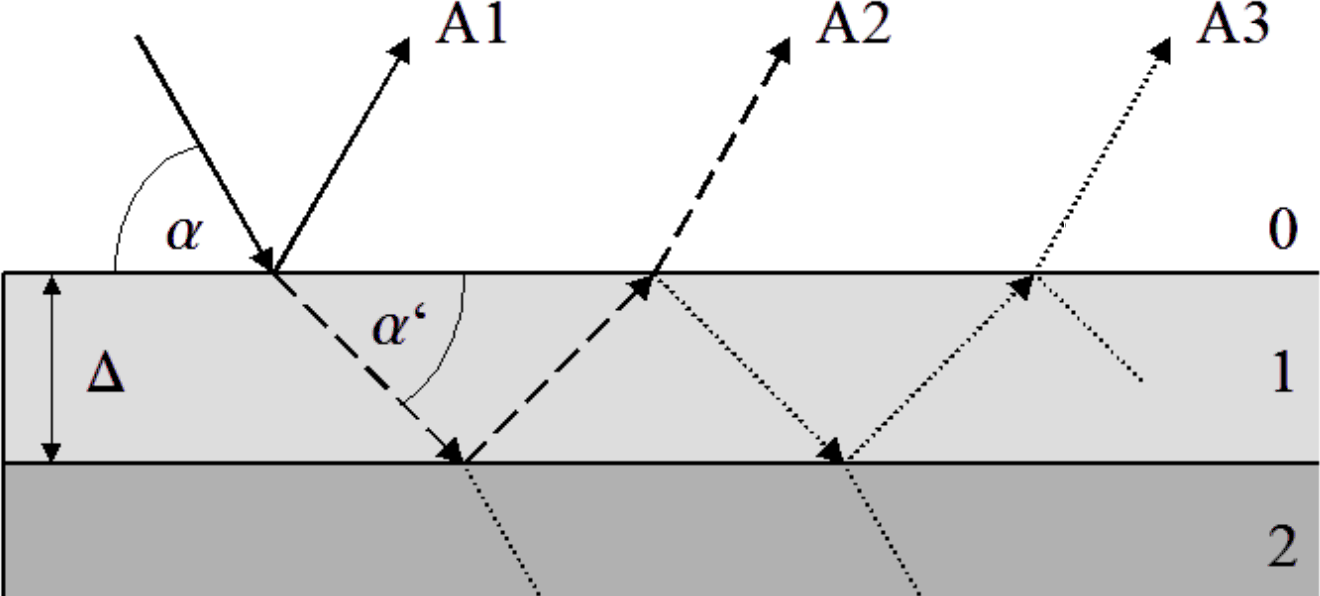
\includegraphics[width=0.6\textwidth]{rontgenreflekt.png}
					\caption{Reflektion an einer Schicht der Dicke $\Delta$ mit Wellenvektor-Übertrag zwischen A1, A2, A3... \cite{USiegenMIE}}
				\end{figure}

			Hierbei ist $\lambda$ die Röntgenstrahlen-Wellenlänge, $r\ix{0}$ der klassische Elektronenradius, $\rho\ix{e}$ die Elektronendichte der Oberflächenstruktur und $\rho\ix{$\infty$}$ die Dichte im Festkörper.\\
			Der Wellenvektor-Übertrag $q\ix{z}$ von einfallender zu reflektierter Welle steht über die \tilt{Bragg-Reflexion} mit der Schicht- bzw. Gitterdicke des reflektierenden Materials $d$ in Zusammenhang (siehe \autoref{eq:vektoruber}). Dieser Übertrag moduliert bzw. quantifiziert die Reflektivität, weswegen aus dem Abstand zweier Maxima $\alpha\ix{m}$ im Transmissionsspektrum auf die Schicht über \autoref{eq:bragg} geschlossen werden kann.

				\begin{align}
					q\ix{z}=&\frac{4\pi\sin\left(\alpha\right)}{\lambda} \label{eq:vektoruber} \\
					d=&\frac{2\pi}{\Delta q\ix{z}}=\frac{m\lambda}{2\sin\left(\alpha\ix{m}\right)} \label{eq:bragg}
				\end{align}

	\newpage
	\section{Durchführung}

		In Vorbereitung auf die Experimente mit Röntgenreflektometrie, AFM und einer Absorptionsspektroskopie (\tilt{UV-Vis}) galt es, verschieden dichte Monoschichten von Goldpartikeln auf Objekt-Trägern abzulagern. Mit Hilfe von positiv geladenen Substraten  (\tilt{PEI} - Polyelktrolyte), welche die Adsorption der negativ geladenen Goldkolloide auf dem Träger aus einer Suspension ermöglichen, wurden für 45 und $\unit[150]{min}$ eine und für $\unit[90]{min}$ zwei Proben hergestellt. Hierbei handelte es sich um aminoterminierte Silane, welche einerseits kovalent an die Glasoberfläche gebunden wurden.\\
		Die Absorptionsspektroskopie bestand aus der Aufnahme von Spektren der unterschiedlichen Goldschichten in verschiedenen Lösungsmitteln bzw. Reinst-Wasser und Luft. Dabei befanden sich besagte Proben wiederum in Glas- bzw. Plastikküvetten. Eine Einzelmessung bestand aus dem Durchgang eines Referenzstrahls durch die freie Versuchskammer und einem durch die Probe, wobei für beide ein Wellenlängen-Spektrum zwischen $\unit[320-720]{nm}$ durchgestimmt wurde.\\
		Im Vorfeld der Röntgenreflektometrie wurde das Goniometer justiert. Anschließend durchlief die Messung einen Winkelbereich von $\unit[0]{\degree}<\theta<\unit[90]{\degree}$, wobei  letzteres einem senkrechten Ein- und Ausfall der Strahlung entsprach. Eine entsprechende Software berechnete aus dem erhaltenen Intensitätsspektrum den Wellenvektor-Übertrag, welcher für die Berechnung der Schichtdicke genutzt werden kann.\\
		Schließlich galt es, die im \tilt{tapping mode} aufgenommen Höhenprofil-Daten der AFM auszuwerten. Eine Bestimmung eines Einzelteilchen-Radius mittels der vorliegenden Software und einer mittleren Dichte wurde vorgenommen.

	\newpage
	\section{Auswertung}

		


	\newpage
	\section{Anhang}

		\bibliography{all.bib}
		\bibliographystyle{unsrt}

\end{document}